\documentclass[main.tex]{subfiles}
\begin{document}
	\begin{titlepage}
		\begin{center}
			\begin{large}
				Санкт-Петербургский политехнический университет\\
				Физико-механический институт\\
				\textbf{Кафедра <<Прикладная математика>>}\\
			\end{large}
			\vfill
			\Large{\textbf{КОНСПЕКТ ЛЕКЦИЙ ПО ДИСЦИПЛИНЕ \\
					<<ДОПОЛНИТЕЛЬНЫЕ ГЛАВЫ СТАТИСТИКИ>>}}
		\end{center}
		\vfill
		\begin{figure}[H]
			% \centering 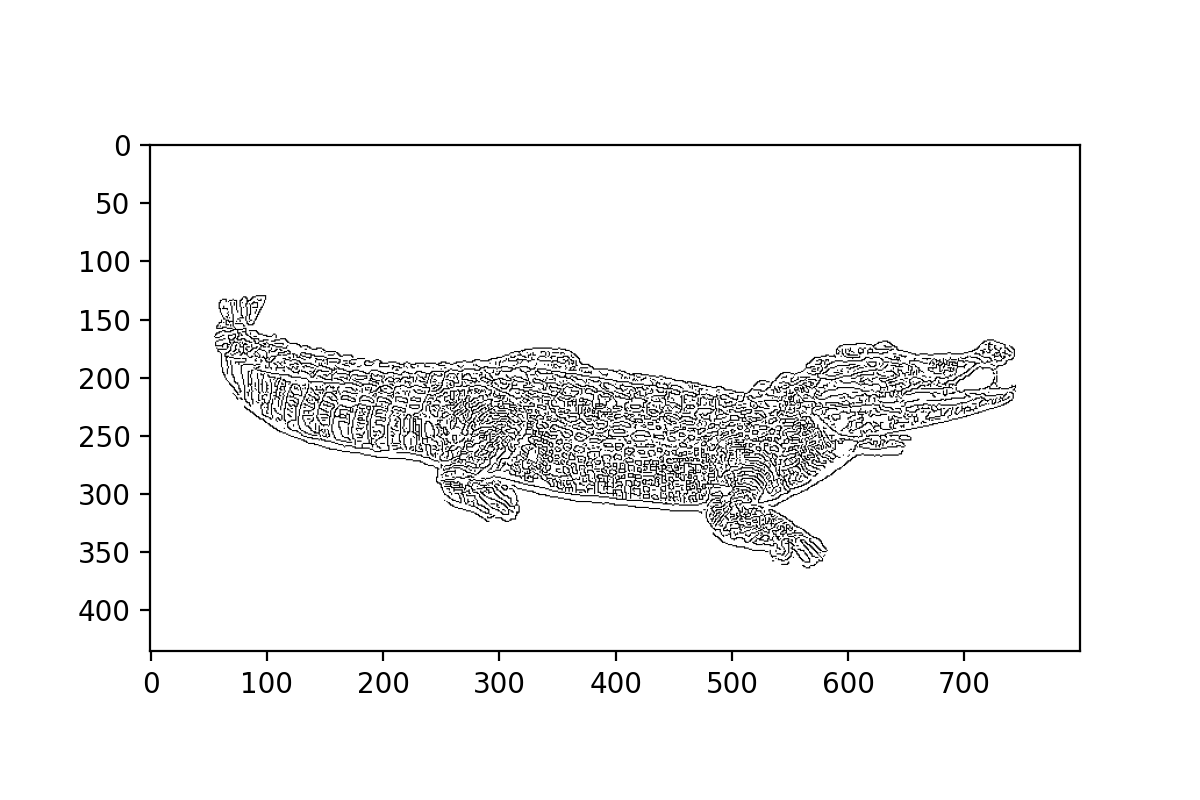
\includegraphics[width=.8\textwidth]{croco_edges}
		\end{figure}
		\vfill
		\centering{Санкт-Петербург \\ 2021}
	\end{titlepage}
\end{document}
